\section{Random Processes}
This chapter concerns mostly with random processes - collection random variables $(X_t)_{t \in T}$, which 
may be dependent. In calssical settings like Brownian motion, $t$ represents time so $T \subset \mathbb{R}$. 
However, in high-dimensional probability $T$ can be any set, and we'll deal with Gaussian processes a lot.

In this chapter, we'll explore powerful comparison inequalities for Gaussian processes - Slepian, 
Sudakov-Frenique, and Gordon - by using a new trick: Gaussian interpolation. Then we use these tools to prove 
a sharp bound on the operator norm of $m \times n$ Gaussian random matrices.

How does a Gaussian process $(X_t)_{t \in T}$ capture the geometry of $T$? We'll prove a lower bound on the 
Gaussian width using covering numbers, and link it to other ideas like effective dimension. Moreover, we'll 
also compute the size of a ranodm projection of any bounded set $T \subset \mathbb{R}^n$, which heavily depends 
on the Gaussian width.



% ----------7.1----------
\subsection{Basic Concepts and Examples}
\begin{definition}[]
\label{def:7.1.1}
A \underline{random process} is a collection of random variables $(X_t)_{t \in T}$ on the same probability 
space, which are indexed by elements $t$ of some index set $T$.
\end{definition}

\begin{example}[Discrete time]
\label{ex:7.1.2}
If $T = \{1, \dots, n\}$ then the random process 
\[ (X_1, \dots, X_n) \]
can be identifies as a random vector in $\mathbb{R}^n$.
\end{example}

\begin{example}[Random walks]
\label{ex:7.1.3}
If $T = \mathbb{N}$, a discrete-time random process $(X_n)_{n \in \mathbb{N}}$ is simply a sequence of random 
variables. An important example is a \textit{random walk} defined as 
\[ X_n := \sum_{i = 1}^{n} Z_i, \]
where the increments $Z_i$ are independent, mean zero random variables. See Figure 7.1 for an illustration:
\begin{center}
	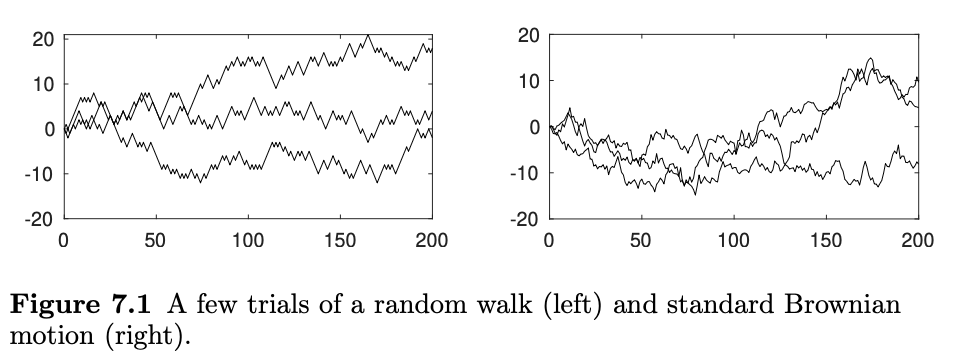
\includegraphics[width=0.8\textwidth]{Chapter 7/fig7-1.png}
\end{center}
\end{example}

\begin{example}[Brownian motion]
\label{ex:7.1.4}
The most classical continuous-time random process is the standard \textit{Brownian motion} $(X_t)_{t \geq 0}$, 
or the \textit{Wiener process}. It can be characterized as follows:
\begin{enumerate}[label={(\roman*)}]
	\item The process has continuous sample paths, i.e. the random function $f(t) := X_t$ is continuous almost 
	surely; 
	\item The increments are independent and satisfy $X_t - X_s \sim N(0, t - s)$ for all $t \geq s$.
\end{enumerate}
Figure 7.1 above also shows some sample paths of a standard Brownian motion.
\end{example}

\begin{example}[Random fields]
\label{ex:7.1.5}
When the index set $T$ is a subset of $\mathbb{R}^n$, a random process $(X_t)_{t \in T}$ is sometimes called a 
spatial random process, or \textit{random field}. For example, the water temperature $X_t$ ar the location on 
Earth that is parameterized by $t$ can be modeled as a spatial random process.
\end{example}


\subsubsection{Covariance and Increments}
In section 3.2, we introduced the covariance matrix of a random vector. Here we'll define the 
\textit{covariance function} of a random process $(X_t)_{t \in T}$ in a similar manner. For simplicity, 
assume the random process has zero mean: 
\[ \mathbb{E}\left[ X_t \right] = 0 \text{ for all } t \in T. \]
The \underline{covariance} function of the process is defined as
\[ \Sigma(t, s) := \mathrm{Cov}(X_t, X_s) = \mathbb{E}\left[ X_tX_s \right], \ t, s \in T. \]
The \underline{increments} of the random process are defined as 
\[ d(t, s) := \lVert X_t - X_s \rVert_{L^2} = (\mathbb{E}\left[ (X_t - X_s)^2 \right])^{1/2}, \ t, s \in T. \]

\begin{example}[]
\label{ex:7.1.6}
The increments of the standard Brownian motion satisfy 
\[ d(t, s) = \sqrt{t - s}, \ t \geq s \]
by definition. The increments of a random walk of \cref{ex:7.1.3} with $\mathbb{E}\left[ Z_i^2 \right] = 1$ 
behave similarly: 
\[ d(n, m) = \sqrt{n - m}, \ n \geq m. \]
\end{example}

\begin{remark}[The canonical metric]
\label{rmk:7.1.7}
Even if the index set $T$ has no geometric structure, the increments $d(t, s)$ always define a metric on $T$, 
thys automatically turning $T$ into a metric space. However, as we see in \cref{ex:7.1.6}, this metric may not 
match the Euclidean distance on $\mathbb{R}^n$.
\end{remark}

\begin{remark}[Covariance v.s. increments]
\label{rmk:7.1.8}
The covariance and the increments contain roughly the same information about the random process. Increments can 
be writeen using the covariance: Just expand the square to see that 
\[ d(t, s)^2 = \Sigma(t, t) - 2 \Sigma(t, s) + \Sigma(s, s). \]
Vise versa, if the zero random variable belongs to the process, we can also recover the covariance from the 
increments (Exercise 7.1).
\end{remark}


\subsubsection{Gaussian Processes}
\begin{definition}[]
\label{def:7.1.9}
A random process $(X_t)_{t \in T}$ is called a \underline{Gaussian process} if, for any finite subset 
$T_0 \subset T$, the random vector $(X_t)_{t \in T_0}$ has a normal distribution. Equivalently, 
$(X_t)_{t \in T}$ is Gaussian if every finite linear combination $\sum_{t \in T_0}^{}a_tX_T$ is a normal random 
variable (Exercise 3.16).
\end{definition}

The notion of Gaussian processes generalized that of Gaussian random vectors in $\mathbb{R}^n$. A classical 
example of a Gaussian process is the standard Brownian motion.

\begin{remark}[Distribution is determined by covariance, increments]
\label{rmk:7.1.10}
The distribution of a mean-zero Gaussian random vector in $\mathbb{R}^n$ is completely determined by its 
covariance matrix (\cref{prop:3.3.5}). The same goes for a mean-zero Gaussian process: its distribution is 
determined by the covariance function $\Sigma(t, s)$, or equivalently by the increments $d(t, s)$, assuming the 
zero variable is part of the process.
\end{remark}

Many tools we learned about random vectors can be applied to random processes. For example, Gaussian 
concentration (\cref{thm:5.2.3}) applies: 
\begin{theorem}[Concentration of Gaussian processes]
\label{thm:7.1.11}
Let $(X_t)_{t \in T}$ be a Gaussian process with finite $T$. Then 
\[ \lVert \sup_{t \in T} X_t - \mathbb{E}\left[ \sup_t X_t \right] \rVert_{\psi_2} 
\leq C \sup_{t \in T} \sqrt{\mathrm{Var}(X_t)}. \]
\end{theorem}

\begin{proof}
Exercise 5.9(b).
\end{proof}

Let's look at a broad class of Gaussian processes indexed by high-dimensional sets $T \subset \mathbb{R}^n$. 
Take a standard normal vector $g \sim N(0, I_n)$ and define 
\[ X_t := \left\langle g, t \right\rangle, \ t \in T. \]
This guves us a Gaussian process $(X_t)_{t \in T}$ called the \textit{canonical Gaussian process}. The 
increments match the Euclidean distance: 
\[ \lVert X_t - X_s \rVert_{L^2} = \lVert t - s \rVert_{2}, \ t, s \in T. \]

Actually, one can realize any Gaussian process as the canonical process above because of the lemma below:
\begin{lemma}[Gaussian random vectors]
\label{lem:7.1.12}
Let $X$ be a mean-zero Gaussian random vector in $\mathbb{R}^n$. Then there exist points $t_1, \dots, t_n$ such 
that 
\[ X \sim (\left\langle g, t_i \right\rangle)_{i = 1}^n, \text{ where } g \sim N(0, I_n). \]
\end{lemma}

\begin{proof}
IF $\Sigma$ denotes the covariance matrix of $X$, then 
\[ X \equiv \Sigma^{1/2}g \text{ where } g \sim N(0, I_n). \]
The entries of $\Sigma^{1/2}g$ are $\left\langle t_i, g \right\rangle$ where the $t_i$ are the rows of 
$\Sigma^{1/2}$. Done!
\end{proof}

It follows that for any Gaussian process $(X_s)_{x \in S}$, all finite-dimensional marginas $(X_s)_{s \in S_0}$, 
$|S_0| = n$ can be represented as the canonical Gaussian process indexed in a certain subset 
$T_0 \subset \mathbb{R}^n$.



% ----------7.2----------
\subsection{Slepian, Sudakov-Fernique, and Gordon Inequalities}
In many applications, it helps to have a \textit{uniform} bound on a random process:
\[ \mathbb{E}\left[ \sup_{t \in T} X_t \right] = ? \]

\begin{remark}[Making \texorpdfstring{$T$}{} finite]
\label{rmk:7.2.1}
To avoid measurability issues, let's think of 
\[ \mathbb{E}\left[ \sup_{t \in T} X_t \right] \text{ as shorthand for } 
\sup_{T_0 \subset T} \mathbb{E}\left[ \max_{t \in T_0} X_t \right] \]
where $T_0$ runs over all finite subsets. The general case usually follows by approximation.
\end{remark}

For some processes, this quantity can be computed exactly. For example, if $(X_t)$ is a standard Brownian 
motion, the so-called reflection principle gives 
\[ \mathbb{E}\left[ \sup_{t \leq t_0} X_t \right] = \sqrt{\frac{2 t_0}{\pi}} \text{ for every } t_0 \geq 0. \]
For general random processes - evern Gaussian - the problem is nontrivial.

The first general bound we prove is the Slepian comparison inequality for Gaussian processes. It basically 
says: the faster the process grows (in terms of the increments), the farther it gets.

\begin{theorem}[Slepian inequality]
\label{thm:7.2.2}
Let $(X_t)_{t \in T}$ and $(Y_t)_{t \in T}$ be two mean zero Gaussian processes. Assume that for all $t, s 
\in T$, we have 
\[ \mathbb{E}\left[ X_t^2 \right] = \mathbb{E}\left[ Y_t^2 \right] \text{ and } 
\mathbb{E}\left[ (X_t - X_s)^2 \right] \leq \mathbb{E}\left[ (Y_t - Y_s)^2 \right]. \]
Then $\sup_{t \in T}X_t$ is stochastically dominated by $\sup_{t \in T}Y_t$: For every $\tau \in \mathbb{R}$, 
\[ P \left( \sup_{t \in T} X_t \geq \tau \right) \leq P \left( \sup_{t \in T} Y_t \geq \tau \right). \]
Consequently, 
\[ \mathbb{E}\left[ \sup_{t \in T} X_t \right] \leq \mathbb{E}\left[ \sup_{t \in T} Y_t \right]. \]
\end{theorem}

We'll provide a proof later in the chapter, as we need some preliminary knowledge on Gaussian interpolation.


\subsubsection{Gaussian Interpolation}
Assume that $T$ is finite; then we can loot at $X = (X_t)_{t \in T}$ and $Y = (Y_t)_{t \in T}$ as Gaussian 
random vectors in $\mathbb{R}^n$ with $n = |T|$. We may also assume that $X$ and $Y$ are independent. 

Define the Gaussian random vector $Z(u)$ in $\mathbb{R}^n$ that continuously interpolates between $Z(0) = Y$ and 
$Z(1) = X$:
\[ Z(u) := \sqrt{u}X + \sqrt{1 - u}Y, \ u \in [0, 1]. \]
Then the covariance matrix of $Z(u)$ continuously interpolates linearly between the covariance matrices of 
$Y$ and $X$: 
\[ \Sigma(Z(u)) = u \Sigma(X) + (1 - u)\Sigma(Y). \]
This is because 
\begin{align*}
	\Sigma(Z(u)) 
	&= \mathbb{E}\left[ Z(u)Z(u)^T \right] \\
	&= \mathbb{E}\left[ (\sqrt{u}X + \sqrt{1 - u}Y)(\sqrt{u}X + \sqrt{1 - u}Y)^T \right] \\
	&= u \mathbb{E}\left[ (X - \mu_X)(X - \mu_X)^T \right] 
	+ \sqrt{u(1 - u)}\mathbb{E}\left[ (X - \mu_X)(Y - \mu_Y)^T \right] \\ 
	&\quad + \sqrt{u(1 - u)}\mathbb{E}\left[ (Y - \mu_Y)(X - \mu_X)^T \right] 
	+ (1 - u) \mathbb{E}\left[ (Y - \mu_Y)(Y - \mu_Y)^T \right] \\
	&= u \Sigma(X) + 0 + 0 + (1 - u)\Sigma(Y) \quad \text{(Independence)} \\
	&= u \Sigma(X) + (1 - u)\Sigma(Y).
\end{align*}

For a given function $f: \mathbb{R}^n \to \mathbb{R}$, let's study how $\mathbb{E}\left[ f(Z(u)) \right]$ 
changes as $u$ increases from 0 to 1. Of special interest to us is the function 
\[ f(x) = \mathbf{1}_{\{\max_{i} x_i < \tau\}}. \]
We'll be able to show that in this case, $\mathbb{E}\left[ f(Z(u)) \right]$ increases in $u$. This would imply 
the conclusion of Slepian inequality, since then 
\[ \mathbb{E}\left[ f(Z(1)) \right] \geq \mathbb{E}\left[ f(Z(0)) \right] 
\implies P \left( \max_{i} X_i < \tau \right) \geq P \left( \max_{i} Y_i < \tau \right) \]
as claimed.

Let's start via the following useful identity:
\begin{lemma}[Gaussian integration by parts]
\label{lem:7.2.3}
Let $X \sim N(0, 1)$. Then for any differentiable function $f: \mathbb{R} \to \mathbb{R}$ we have 
\[ \mathbb{E}\left[ Xf(X) \right] = \mathbb{E}\left[ f'(X) \right]. \]
\end{lemma}

\begin{proof}
Assume first that $f$ has bounded support. Denoting the Gaussian density by 
\[ p(x) = \frac{1}{\sqrt{2 \pi}}e^{-x^2 / 2}, \]
we can express the expectation as an integral, and integrate it by parts:
\begin{align*}
	\mathbb{E}\left[ f'(X) \right] 
	&= \int_{\mathbb{R}}^{} f'(x)p(x) \ dx \\
	&= [f(x)p(x)]_{-\infty}^\infty - \int_{\mathbb{R}}^{} f(x)p'(x) \ dx \\
	&= 0 - \int_{\mathbb{R}}^{} f(x)p'(x) \ dx \\
	&= - \int_{\mathbb{R}}^{} f(x)p'(x) \ dx.
\end{align*}
We have already proved before (Exercise 2.3) that $p'(x) = -xp(x)$, hence the integral above equals 
\[ \int_{\mathbb{R}}^{} f(x)p(x)x \ dx = \mathbb{E}\left[ Xf(X) \right], \]
as claimed. The result can be extended to general functions by an approximation argument. The lemma is proved.
\end{proof}

By rescaling, we can extend Gaussian integration by parts for $X \sim N(0, \sigma^2)$: 
\[ \mathbb{E}\left[ Xf(X) \right] = \sigma^2 \mathbb{E}\left[ f'(X) \right]. \]
(Just write $X = \sigma Z$ for $Z \sim N(0, 1)$ and apply \cref{lem:7.2.3}). We can also extend it to high 
dimensions: 

\begin{lemma}[Multivariate Gaussian integration by parts]
\label{lem:7.2.4}
Let $X \sim N(0, \Sigma)$. Then for any differentiable function $f: \mathbb{R}^n \to \mathbb{R}$ we have 
\[ \mathbb{E}\left[ Xf(X) \right] = \Sigma \cdot \mathbb{E}\left[ \nabla f(X) \right] \]
assuming both expectations are finite. In other words, 
\[ \mathbb{E}\left[ X_i f(X) \right] = \sum_{j = 1}^{n} \Sigma_{ij} 
\mathbb{E}\left[ \frac{\partial f}{\partial x_j}(X) \right], \ i = 1, \dots, n. \]
\end{lemma}

\begin{proof}
Exercise 7.6.
\end{proof}

\begin{lemma}[Gaussian interpolation]
\label{lem:7.2.5}
Consider two independent Gaussian random vectors $X \sim N(0, \Sigma^X)$ and $Y \sim N(0, \Sigma^Y)$. Define 
the interpolation Gaussian vector 
\[ Z(u) := \sqrt{u}X + \sqrt{1 - u}Y, \ u \in [0, 1]. \]
Then for any twice differentiable function $f: \mathbb{R}^n \to \mathbb{R}$, we have
\[ \frac{d}{du}\mathbb{E}\left[ f(Z(u)) \right] = \frac{1}{2}\sum_{i, j = 1}^{n}(\Sigma_{ij}^X - \Sigma_{ij}^Y) 
\mathbb{E}\left[ \frac{\partial^2 f}{\partial x_i \partial x_j}(Z(u)) \right], \]
assuming all expectations exist and are finite.
\end{lemma}

\begin{proof}
Using the multivariate chain rule, 
\begin{align*}
	\frac{d}{du}\mathbb{E}\left[ f(Z(u)) \right] 
	&= \sum_{i = 1}^{n} \mathbb{E}\left[ \frac{\partial f}{\partial x_i}(Z(u)) \frac{dZ_i}{du} \right] \\
	&= \frac{1}{2}\sum_{i = 1}^{n} \mathbb{E}\left[ \frac{\partial f}{\partial x_i}(Z(u)) 
	\left( \frac{X_i}{\sqrt{u}} - \frac{Y_i}{\sqrt{1 - u}} \right) \right].
\end{align*}
Let's break the sum above into two, and first compute the contribution of the terms containing $X_i$. To this 
end, we condition on $Y$ and express 
\[ \sum_{i = 1}^{n}\frac{1}{\sqrt{u}} \mathbb{E}\left[ X_i \frac{\partial f}{\partial x_i}(Z(u)) \right] 
= \sum_{i = 1}^{n} \frac{1}{\sqrt{u}} \mathbb{E}\left[ X_i g_i(X) \right] \quad (*), \]
where 
\[ g_i(X) = \frac{\partial f}{\partial x_i}(\sqrt{u}X + \sqrt{1 - u}Y). \]
Apply the multivariate Gaussian integration by parts (\cref{lem:7.2.4}), we get 
\begin{align*}
	\mathbb{E}\left[ X_ig_i(X) \right] 
	&= \sum_{j = 1}^{n} \Sigma_{ij}^X \mathbb{E}\left[ \frac{\partial g_i}{\partial x_j}(X) \right] \\
	&= \sum_{j = 1}^{n} \Sigma_{ij}^X \mathbb{E}\left[ \frac{\partial^2 f}{\partial x_i \partial x_j} 
	(\sqrt{u}X + \sqrt{1 - u}Y) \right] \cdot \sqrt{u}.
\end{align*}
Substituting this into $(*)$ to get 
\[ \sum_{i = 1}^{n} \frac{1}{\sqrt{u}} \mathbb{E}\left[ X_i \frac{\partial f}{\partial x_i}(Z(u)) \right] 
= \sum_{i, j = 1}^{n} \Sigma_{ij}^X \mathbb{E}\left[ \frac{\partial^2 f}{\partial x_i \partial x_j}(Z(u))
\right]. \]
Taking expectations on both sides with respect to $Y$, we left the conditioning on $Y$. 

We can similarly evaluate the other sum (terms containing $Y_i$) by conditioning on $X$. Combining the two 
sums we complete the proof.
\end{proof}


\subsubsection{Proof of Slepian Inequality}
We'll establish a preliminary, functional form of Spelian's inequality first:

\begin{lemma}[Slepian inequality, functional form]
\label{lem:7.2.6}
Consider two mean zero Gaussian random vectors $X, Y$ in $\mathbb{R}^n$. Assume that for all $i, j = 1, \dots
, n$, we have 
\[ \mathbb{E}\left[ X_i^2 \right] = \mathbb{E}\left[ Y_i^2 \right] \text{ and } 
\mathbb{E}\left[ (X_i - X_j)^2 \right] \leq \mathbb{E}\left[ (Y_i - Y_j)^2 \right]. \]
Consider a twice-differentiable function $f: \mathbb{R}^n \to \mathbb{R}$ such that 
\[ \frac{\partial^2 f}{\partial x_i \partial x_j} \geq 0 \text{ for all } i, j. \]
Then 
\[ \mathbb{E}\left[ f(X) \right] \geq \mathbb{E}\left[ f(Y) \right], \]
assuming both expectations exist and are finite.
\end{lemma}

\begin{proof}
The assumptions imply that the entries of the covariance matrices $\Sigma^X$ and $\Sigma^Y$ satisfy 
\[ \Sigma_{ii}^X = \Sigma_{ii}^Y \text{ and } \Sigma_{ij}^X \geq \Sigma_{ij}^Y \]
for all $i, j = 1, \dots, n$. We can assume that $X$ and $Y$ are independent. Apply \cref{lem:7.2.5} and using 
our assumptions, we conclude that 
\[ \frac{d}{du}\mathbb{E}\left[ f(Z(u)) \right] \geq 0, \]
so $\mathbb{E}\left[ f(Z(u)) \right]$ increases in $u$. Then $\mathbb{E}\left[ f(Z(1)) \right] = 
\mathbb{E}\left[ f(X) \right]$ is at least as large as $\mathbb{E}\left[ f(Z(0)) \right] 
= \mathbb{E}\left[ f(Y). \right]$. This completes the proof.
\end{proof}

Now we are ready to prove Slepian's inequality (\cref{thm:7.2.2}). Let's state and prove it in the equivalent 
form for Gaussian random vectors.

\begin{theorem}[Slepian inequality]
\label{thm:7.2.7}
Let $X, Y$ be Gaussian random vectors as in \cref{lem:7.2.6}. Then for every $\tau \geq 0$ we have 
\[ P \left( \max_{i \leq n} X_i \geq \tau \right) \leq P \left( \max_{i \leq n} Y_i \geq \tau \right). \]
Consequently, 
\[ \mathbb{E}\left[ \max_{i \leq n}X_i \right] \leq \mathbb{E}\left[ \max_{i \leq n}X_i \right]. \]
\end{theorem}

\begin{proof}
Let $h: \mathbb{R} \to [0, 1]$ be a twice-differentiable, non-increasing approximation to the indicator function 
on the interval $(-\infty, \tau)$: 
\[ h(x) \approx \mathbf{1}_{\{-\infty, \tau\}}, \]
like in Figure 7.2 below.
\begin{center}
    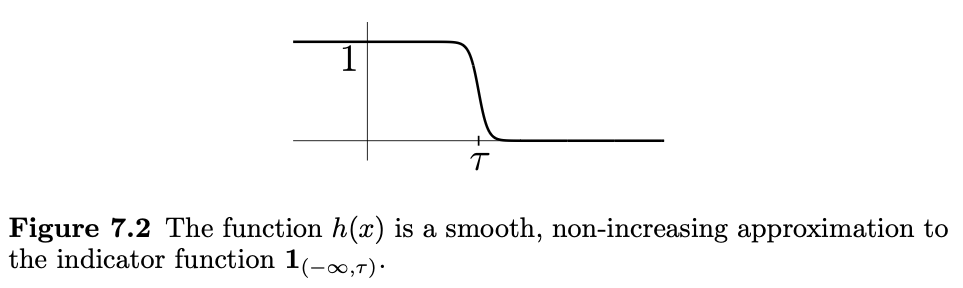
\includegraphics[width=0.8\textwidth]{Chapter 7/fig7-2.png}
\end{center}
Define the function $f: \mathbb{R}^n \to \mathbb{R}$ by 
\[ f(x) = h(x_1) \cdots h(x_n) = \prod_{i = 1}^{n} h(x_i). \]
Then $f(x)$ is an approximation to the indicator function 
\[ f(x) \approx \mathbf{1}_{\{\max_{i}x_i < \tau\}}. \]
We are looking to apply the functional form of Slepian inequality (\cref{lem:7.2.6}) for $f(x)$.

To check the assumptions of this result, note that for $i \neq j$ we have 
\[ \frac{\partial^2 f}{\partial x_i \partial x_j} = h'(x_i) h'(x_j) \cdot \prod_{k \notin \{i, j\}}^{} h(x_k). \]
The first two terms are non-positive and the others are nonnegative by assumption, hence the second derivative 
is nonnegative, as required. It follows that 
\[ \mathbb{E}\left[ f(X) \right] \geq \mathbb{E}\left[ f(Y) \right]. \]
By approximation, it implies 
\[ P \left( \max_{i \leq n} X_i < \tau \right) \geq P \left( \max_{i \leq n} Y_i < \tau \right). \]
This proves the first part. The second part follows by using the integrated tail formula in Exercise 1.15 (b):
\[ \mathbb{E}\left[ f(X) \right] 
= \int_{0}^{\infty} P \left( \max_{i \leq n} X_i \geq \tau \right) \ d \tau 
\leq \int_{0}^{\infty} P \left( \max_{i \leq n} Y_i \geq \tau \right) \ d \tau = \mathbb{E}\left[ f(Y) \right]. \]
\end{proof}


\subsubsection{Sudakov-Fernique and Gordon Inequalities}
Slepian inequality has two assumptions on the processes $(X_t)$ and $(Y_t)$: the equality of varainces and the 
dominance of increments. We now remove the assumption on the equality of variances:

\begin{theorem}[Sudakov-Fernique inequality]
\label{thm:7.2.8}
Let $(X_t)_{t \in T}$ and $(Y_t)_{t \in T}$ be two mean zero Gaussian processes. Assume that for all $t, s 
\in T$, we have 
\[ \mathbb{E}\left[ (X_t - X_s)^2 \right] \leq \mathbb{E}\left[ (Y_t - Y_s)^2 \right]. \]
Then 
\[ \mathbb{E}\left[ \sup_{t \in T}X_t \right] \leq \mathbb{E}\left[ \sup_{t \in T}Y_t \right]. \]
\end{theorem}

\begin{proof}
It is enough to prove this for Gaussian random vectors $X$ and $Y$ in $\mathbb{R}^n$, just like we did for 
Slepian's inequality in \cref{thm:7.2.7}. 

We again deduce the result from Gaussian Interpolation (\cref{lem:7.2.5}). But this time, we'll approximate 
$f(x) \approx \max_{i} x_i$. Let $\beta > 0$ be a parameter and define the function 
\[  f(x) := \frac{1}{\beta}\log_{}{\sum_{i = 1}^{n} e^{\beta x_i}}. \]
We can check that indeed 
\[ \lim_{\beta \to \infty} f(x) = \max_{i = 1, \dots, n}x_i. \]
Substituting $f(x)$ into the Gaussian interpolation formula and simplifying shows that (Exercise 7.7)
\[ \frac{d}{du}\mathbb{E}\left[ f(Z(u)) \right] \leq 0 \text{ for all } u \in [0, 1]. \]
Then we can finish the proof just like in Slepian's inequality.
\end{proof}

Gordon's inequality extends the Slepian and Sudakov-Frenique inequalities to the min-max setting:

\begin{theorem}[Gordon's inequality]
\label{thm:7.2.9}
Let $(X_{ut})_{u \in U, t \in T}$ and $(Y_{ut})_{u \in U, t \in T}$ be two mean-zero Gaussian processes indexed 
by pairs of points $(u, t)$ in a product set $U \times T$. Assume that 
\begin{align*}
	\mathbb{E}\left[ (X_{ut} - X_{us})^2 \right] \leq \mathbb{E}\left[ (Y_{ut} - Y_{us})^2 \right] 
	&\text{ for all } u, t, s; \\
	\mathbb{E}\left[ (X_{ut} - X_{vs})^2 \right] \geq \mathbb{E}\left[ (Y_{ut} - Y_{vs})^2 \right] 
	&\text{ for all } u \neq v \text{ and all } t, s.
\end{align*}
Then for every $\tau \geq 0$, 
\[ P \left( \inf_{u \in U}\sup_{t \in T} X_{ut} \geq \tau \right) 
\leq P \left( \inf_{u \in U}\sup_{t \in T} Y_{ut} \geq \tau \right). \]
Moreover, by the integrated tail formula, 
\[ \mathbb{E}\left[ \inf_{u \in U}\sup_{t \in T} X_{ut} \right] \leq 
\mathbb{E}\left[ \inf_{u \in U}\sup_{t \in T} Y_{ut} \right]. \]
\end{theorem}

\begin{proof}
The proof under the additional assumption of equal variances is in Exercise 7.9. The proof for this statement 
is much harder.
\end{proof}



% ----------7.3----------
\subsection{Application: Sharp Bounds for Gaussian Matrices}



% ----------7.4----------
\subsection{Sudakov Inequality}
Recall that for a general mean-zero Gaussian process $(X_t)_{t \in T}$ on some index set $T$, the increments 
\[ d(t, s) := \lVert X_t - X_s \rVert_{L^2} = (\mathbb{E}\left[ (X_t - X_s)^2 \right])^{1/2} \]
define a metric on $T$, called the \textit{canonical metric}. This metric determines the covariance function 
$\Sigma(t, s)$, which in turn determines the distribution of the proces $(X_t)_{t \in T}$ (\cref{rmk:7.1.10}). 
So, in theory, we can ask any question about the distribution of the process by understanding the geometry of 
the metric space $(T, d)$ - studying probability via geometry!

Now the question comes: How can we estimate 
\[ \mathbb{E}\left[ \sup_{t \in T} X_t \right] \]
in terms of the geometry of $(T, d)$? This is a hard problem we will study from now well into Chapter 8.

We'll start with a lower bound in terms of the \textit{metric entropy}, which was introduced in Chapter 4. 
Recall that for any $\varepsilon > 0$, the \textit{covering number} 
\[ \mathcal{N}(T, d, \varepsilon) \]
is the samllest cardinality of an $\varepsilon$-net of $T$ in the metric $d$, or equivalently the smallest 
number of closed balls of radius $\varepsilon$ whose union covers $T$. The logarithm of the of the covering 
number, $\log_{2}{\mathcal{N}(T, d, \varepsilon)}$, is called the \textit{metric entropy} ot $T$.

\begin{theorem}[Sudakov's inequality]
\label{thm:7.4.1}
Let $(X_t)_{t \in T}$ be a mean-zero Gaussian process. Then, for any $\varepsilon \geq 0$, we have 
\[ \mathbb{E}\left[ \sup_{t \in T} X_t \right] \geq c \varepsilon \sqrt{\log_{}{\mathcal{N}(T, d, 
\varepsilon)}} \]
where $d$ is the canonical metric defined above.
\end{theorem}

\begin{proof}
We'll deduce the result from the Sudakov-Frenique comparison inequality (\cref{thm:7.2.8}). Assume that 
\[ N := \mathcal{N}(T, d, \varepsilon) \]
is finite; the infinite case is in Exercise 7.14. Let $\mathcal{N}$ be a maximal $\varepsilon$-seperated subset 
of $T$. Then $\mathcal{N}$ is an $\varepsilon$-net of $T$ (\cref{lem:4.2.6}), and thus 
\[ |\mathcal{N}| \geq N. \]
Restricting the process to $\mathcal{N}$, we see that it suffices to show that 
\[ \mathbb{E}\left[ \sup_{t \in \mathcal{N}} X_t \right] \geq c \varepsilon \sqrt{\log_{}{N}}. \]
Let's do it by comparing $(X_t)_{t \in \mathcal{N}}$ to a simpler Gaussian process $(Y_t)_{t \in \mathcal{N}}$, 
defined as follows: 
\[ Y_t := \frac{\varepsilon}{\sqrt{2}}g_t \text{ where } g_t \sim_{i.i.d.} N(0, 1). \]
To use the Sudakov-Fernique comparison inequality (\cref{thm:7.2.8}), we need to compare the increments of 
the two processes. Fix two different points $t, s \in \mathcal{N}$. By definition, 
\[ \mathbb{E}\left[ (X_t - X_s)^2 \right] = d(t, s)^2 \geq \varepsilon^2 \]
while 
\[ \mathbb{E}\left[ (Y_t - Y_s)^2 \right] = \frac{\varepsilon^2}{2}\mathbb{E}\left[ (g_t - g_s)^2 \right] = 
\varepsilon^2 \quad (g_t - g_s \sim N(0, 2)). \]
This implies that 
\[ \mathbb{E}\left[ (X_t - X_s)^2 \right] \geq \mathbb{E}\left[ (Y_t - Y_s)^2 \right] \text{ for all } 
t, s \in \mathcal{N}. \]
By applying \cref{thm:7.2.8}, we obtain 
\[ \mathbb{E}\left[ \sup_{t \in \mathcal{N}}X_t \right] \geq \mathbb{E}\left[ \sup_{t \in \mathcal{N}}X_t 
\right] = \frac{\varepsilon}{2}\mathbb{E}\left[ \max_{t \in \mathcal{N}}g_t \right] 
\geq c \varepsilon \sqrt{\log_{}{N}}. \]
In the last step, we used that the expected maximum of $N$ i.i.d $N(0, 1)$ random variables is at least 
$c \sqrt{\log_{}{N}}$ (Exercise 2.38 (b)). The proof is complete.
\end{proof}


\subsubsection{Application for covering numbers in \texorpdfstring{$\mathbb{R}^n$}{}}
Sudakov's inequality can be used to bound the covering numbers of an arbitrary set $T \subset \mathbb{R}^n$: 

\begin{corollary}[Sudakov inequality in \texorpdfstring{$\mathbb{R}^n$}{}]
\label{cor:7.4.2}
Let $T \subset \mathbb{R}^n$. Then for any $\varepsilon > 0$, 
\[ \mathbb{E}\left[ \sup_{t \in T} \left\langle g, t \right\rangle \right] 
\geq c \varepsilon \sqrt{\log_{}{\mathcal{N}(T, \varepsilon)}}, \]
where $\mathcal{N}(T, \varepsilon)$ just the covering number of $T$.
\end{corollary}

\begin{proof}
Consider the canonical Gaussian process $X_t := \left\langle g, t \right\rangle$ where $g \sim N(0, I_n)$. As 
we noted in Section 7.1.2, the canonical distance for this process is the Euclidean distance in $\mathbb{R}^n$, 
i.e. 
\[ d(t, s) = \lVert X_t - X_s \rVert_{L^2} = \lVert t - s \rVert_{2} \text{ for any } t, s \in T. \]
Then the corollary directly follows from Sudakov's inequality (\cref{thm:7.4.1}).
\end{proof}

Aside from the bound above, \cref{cor:7.4.2} is also sharp up to a log factor (Exercise 8.5): 
\[ \mathbb{E}\left[ \sup_{t \in T}\left\langle g, t \right\rangle \right] 
\leq C \log_{}{(n)} \cdot \varepsilon \sqrt{\log_{}{\mathcal{N}(T, \varepsilon)}}. \]

For a quick application of Sudakov's inequality, let's (roughly) re-derive the boudne on covering numbers of 
polytopes in $\mathbb{R}^n$ from \cref{cor:0.1.1}: 

\begin{corollary}[Covering numbers of polytopes]
\label{cor:7.4.3}
Let $P$ be a polytope in $\mathbb{R}^n$ with $N$ vertices, contained in the unit Euclidean ball. Then for 
every $\varepsilon > 0$, we have
\[ \mathcal{N}(P, \varepsilon) \leq N^{C / \varepsilon^2}. \]
\end{corollary}

\begin{proof}
If $x_1, \dots, X_N$ are the vertices of $P$, then 
\[ \mathbb{E}\left[ \sup_{t \in P}\left\langle g, t \right\rangle \right] 
\leq \mathbb{E}\left[ \sup_{i = 1, \dots, N}\left\langle g, x_i \right\rangle \right] \leq 
C \sqrt{\log_{}{N}}. \]
The first bound follows from the maximal principle (Exercise 1.4): Since $P$ lies the convex hull of its 
vertices, for each fixed $g$, the linear (and thus convex) function $t \mapsto \left\langle g, t \right\rangle$ 
attains its maximum at a vertex. The second bound is due to the maximal inequality from \cref{prop:2.7.6}, 
as $\left\langle g, x \right\rangle \sim N(0, \lVert x \rVert_{2}^2)$ and $\lVert x \rVert_{2} \leq 1$. 
Substitute this into \cref{cor:7.4.2} and simplify completes the proof.
\end{proof}



% ----------7.5----------
\subsection{Gaussian Width}
From the previous subsection, we saw an important quantity associated with any set $T \subset \mathbb{R}^n$: 
the size of the canonical Gaussian process on $T$. It shows up a lot in high-dimensional probability, so 
let's give it a name and look at its basic properties.

\begin{definition}[]
\label{def:7.5.1}
The \underline{Gaussian width} of a subset $T \subset \mathbb{R}^n$ is defined as 
\[ w(T) := \mathbb{E}\left[ \sup_{t \in T}\left\langle g, x \right\rangle \right] \text{ where } 
g \sim N(0, I_n). \]
\end{definition}

Try to think of Gaussian width as a fundamental geometric measure of a set $T \subset \mathbb{R}^n$, like 
volume or surface area.





% ----------7.6----------
\subsection{Application: Random Projection of Sets}
